\paragraph{Ground Wire} Multiple sources insist that a ground wire is necessary between the stimulating and recording electrodes~\cite{StahlMSEE,Olivo,KuehJellies,EllingerMSEE,Kladt2010}.  In~\cite{Olivo}, it is suggested that one of the dissecting pins may be connected to ground.  In~\cite{Kladt2010}, which is an experiment in which the earthworm is not dissected, a piece of aluminium foil is placed on the earthworm body and connected to ground.  \cite{KuehJellies} implies that a chlorided silver wire is placed under the body of earthworm and connected to ground; this is illustrated in figures~\ref{fig:EWSetup} and~\ref{fig:EWSetupPA}, and it is the setup used to achieve the results in section~\ref{sec:app}.

In some of the first attempts at the experiment, I used a general purpose tin or nickel (I'm not sure which) plated solid copper core hookup wire stripped of its insulation and placed under the earthworm body and connected to ground.  With the plated copper wire, I saw 60Hz noise coming out of the Preamp connected to the recording electrodes.  Switching to chlorided silver wire for the ground wire under the earthworm eliminated the problem.  It was suggested to me by either Dr. Miller or Mr. Mike Ellinger that copper is toxic to cells and should certainly not be used for the recording electrodes, but it seems that plated copper wire should not be used for the ground wire.  It may also be that the tin or nickel plating is toxic to the worm (this is only my supposition).  \cite{Olivo} and~\cite{Kladt2010} appear to successfully use a steel pin and aluminium foil, respectively, as the ground ``wire.''

\paragraph{Response Abnormalities} Another issue that appeared in our attempts at recreating the experiment with earthworm giant axons described in~\cite{StahlMSEE,Olivo,KuehJellies,EllingerMSEE} was trying to recreate the shape (biphasic) and amplitude.  This issue was unrelated to the DASS hardware, specifically, as much of this behavior was observed with a commercial stimulator and a Preamp board from~\cite{BatzerCorsiCrampton}.

The expected biphasic (0V to positive to 0V to negative to 0V) shape of the combined action potentials along the nerve cord, as seen in the lateral response in figure~\ref{fig:EWLatResp}, is due to the relative polarization on the nerve cord between the recording electrodes~\cite{KuehJellies,McGillCAP}.  It is a coincidence that the combined action potential resembles the membrane voltage during a single action potential response.  It was somewhat disconcerting to see that the median response in figures~\ref{fig:EWMedResp} and~\ref{fig:EWLatResp} was monophasic (0V to positive to 0V).  Although, monophasic median and lateral responses were also observed in figure 32 of~\cite{StahlMSEE}.  Also,~\cite{McGillCAP} concerns a similar experiment with the sciatic nerve of a frog, and it says that a nerve cord that is crushed at one of the recording electrode will result in a monophasic response measurement.  I hypothesize that a similar phenomenon could occur in the earthworm's nerve cord.

We also experienced inconsistent results in the amplitude of the response waveforms.  The position of the recording electrodes will affect the amplitude of the response: recording electrodes placed further apart will result in a lower amplitude, as reported in~\cite{KuehJellies,McGillCAP}.  Consequently, it is expected that the responses measure with different earthworms will have different amplitudes.  But, we experienced varying amplitudes with the same worm.   One thing we observed was that when using the commercial Grass SD9 Stimulator set to send stimulation pulses at the same level about 1-5 times per second, the amplitude of the response waveforms were consistent.  If the stimulation were turned off for a time and turned back on, the amplitude of the response would be different.  This causes inconsistent response amplitudes when using the DASS because stimulation pulses are not happening at a consistent rate: the script run on the DASCC might be set to send one stimulation pulse at some amplitude, the results analyzed by the operator, the stimulation amplitude adjusted, and then another stimulation pulse sent.  This means that stimulation pulses are sent at irregular intervals with minutes in between pulses.  Moistening the nerve cord also changed the response amplitude.

Large stimulation artifacts that did not settle before the median response occurred (figure~\ref{fig:settle}), abnormal (not mono or bi-phasic) shapes (figure~\ref{fig:abnormal}), and multiple apparent responses from one stimulus (figure~\ref{fig:multi}) also appeared in the early experiments.  As the issues were being investigated, I focused on improving the biological experimental technique.  Keeping the nerve cord moist with Ringer's solution (as suggested by~\cite{Olivo,KuehJellies}) while also keeping the amount of solution collecting around the worm to a minimum (by wicking excess solution away with paper towel) appears to have kept the aforementioned issues from happening again (since the Aug. 10, 2012 experiments).

\begin{figure}[H]
	\centering 
	\begin{singlespace}
	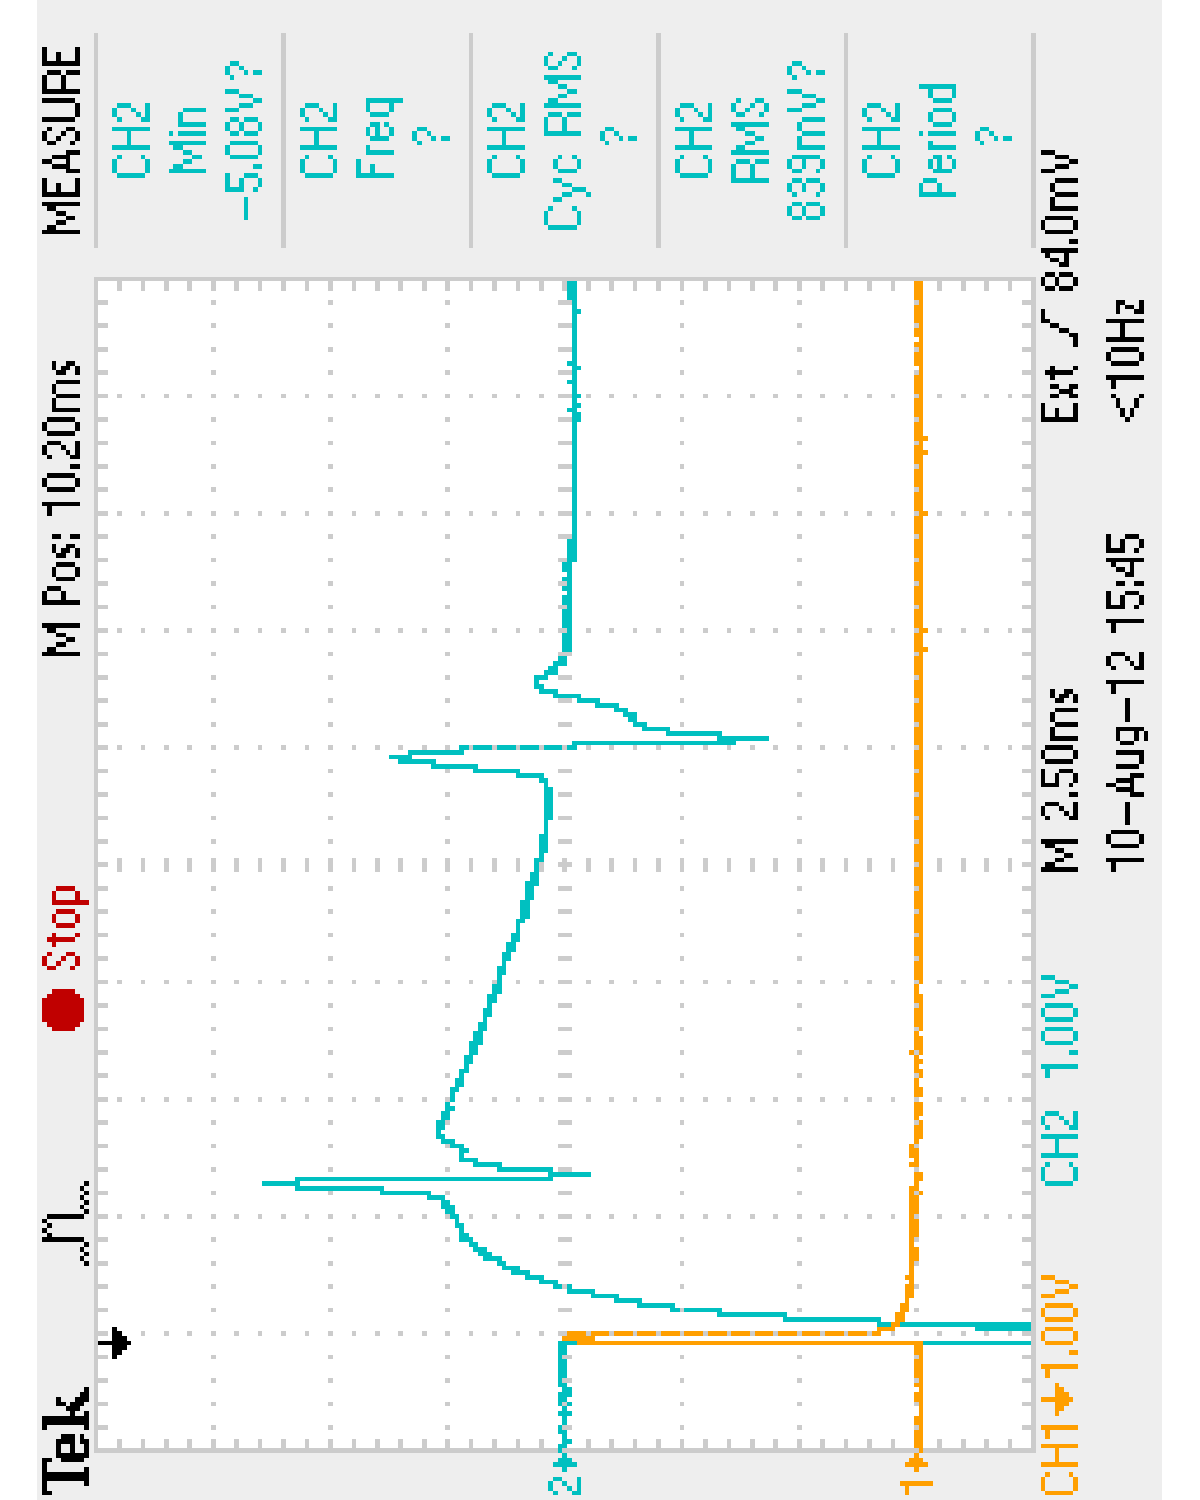
\includegraphics[trim=0 0.1in 0 0.1in,clip,angle=-90,width=0.48\textwidth]{./figures/F0002TEK_settle_120810} %[trim=left bottom right top]
	\caption{ALL0002 Aug. 10, 2012; long stimulus artifact settling time\label{fig:settle}}
	\end{singlespace}
\end{figure}

\begin{figure}[H]
	\centering 
	\begin{singlespace}
	\begin{subfigure}[b]{0.48\textwidth}
		\centering 
		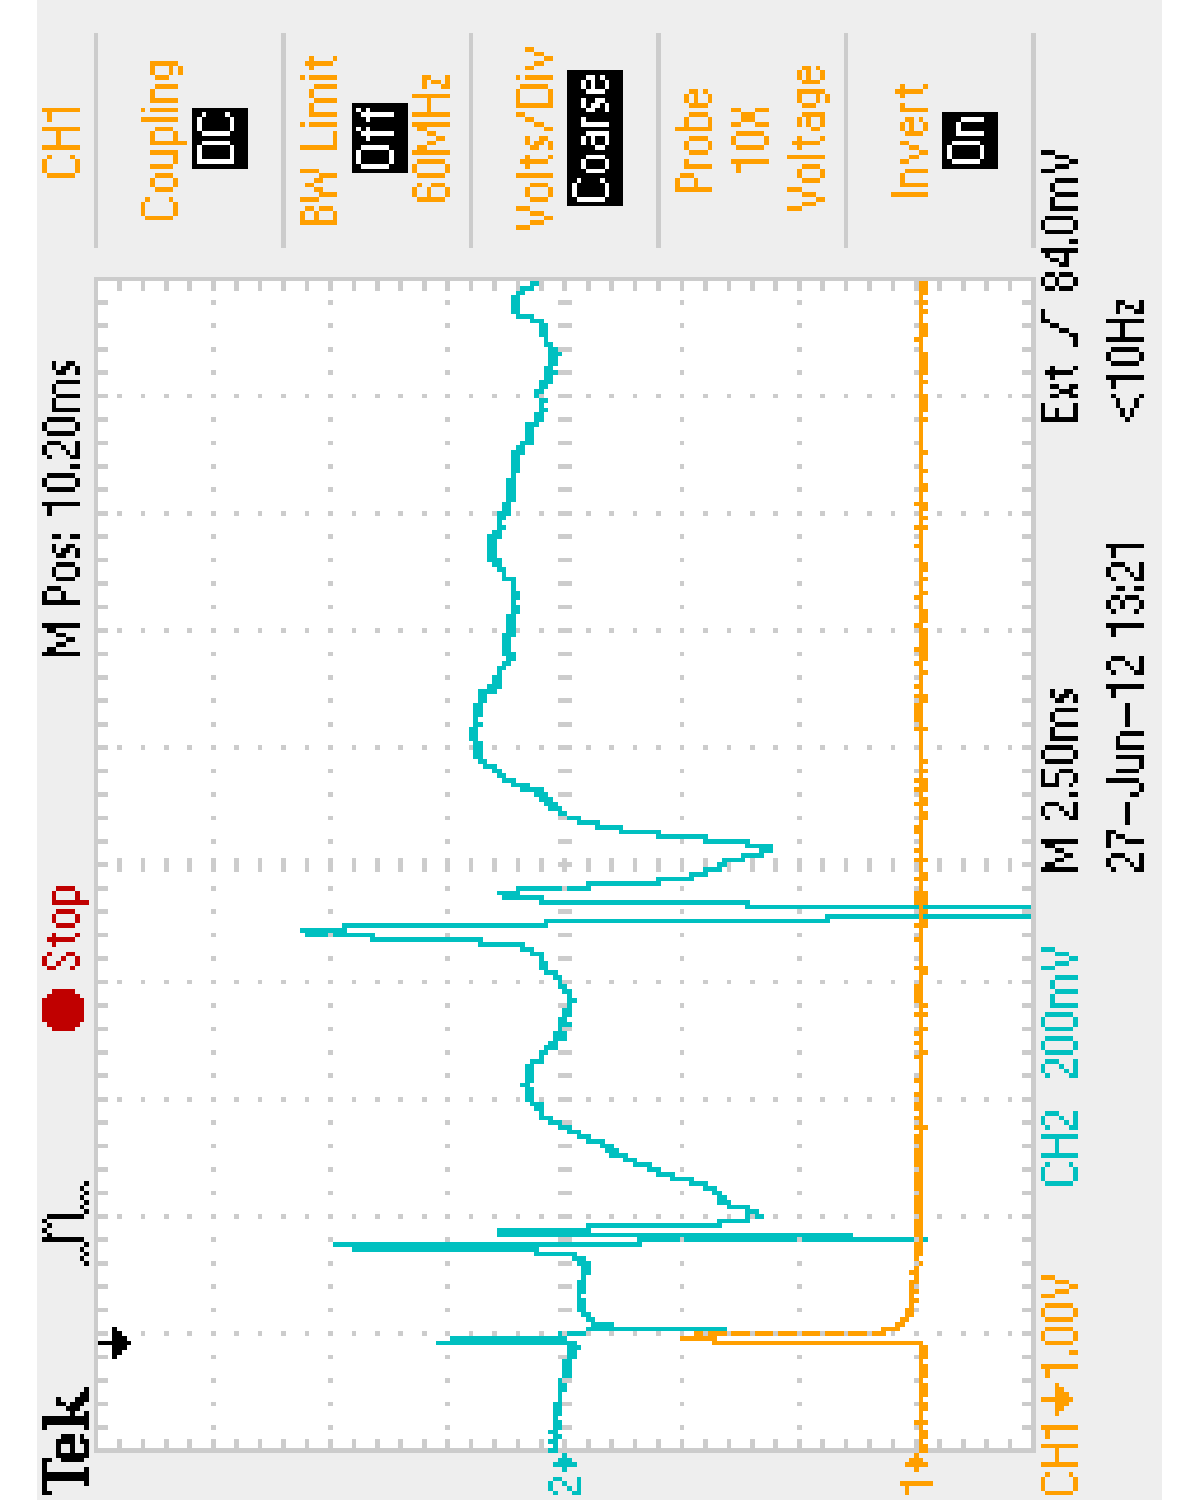
\includegraphics[trim=0 0.1in 0 0.1in,clip,angle=-90,width=\textwidth]{./figures/F0000TEK_abnorm_120627} %[trim=left bottom right top]
	\caption{ALL0000 June 27, 2012}
	\end{subfigure}
	~
	\begin{subfigure}[b]{0.48\textwidth}
		\centering 
		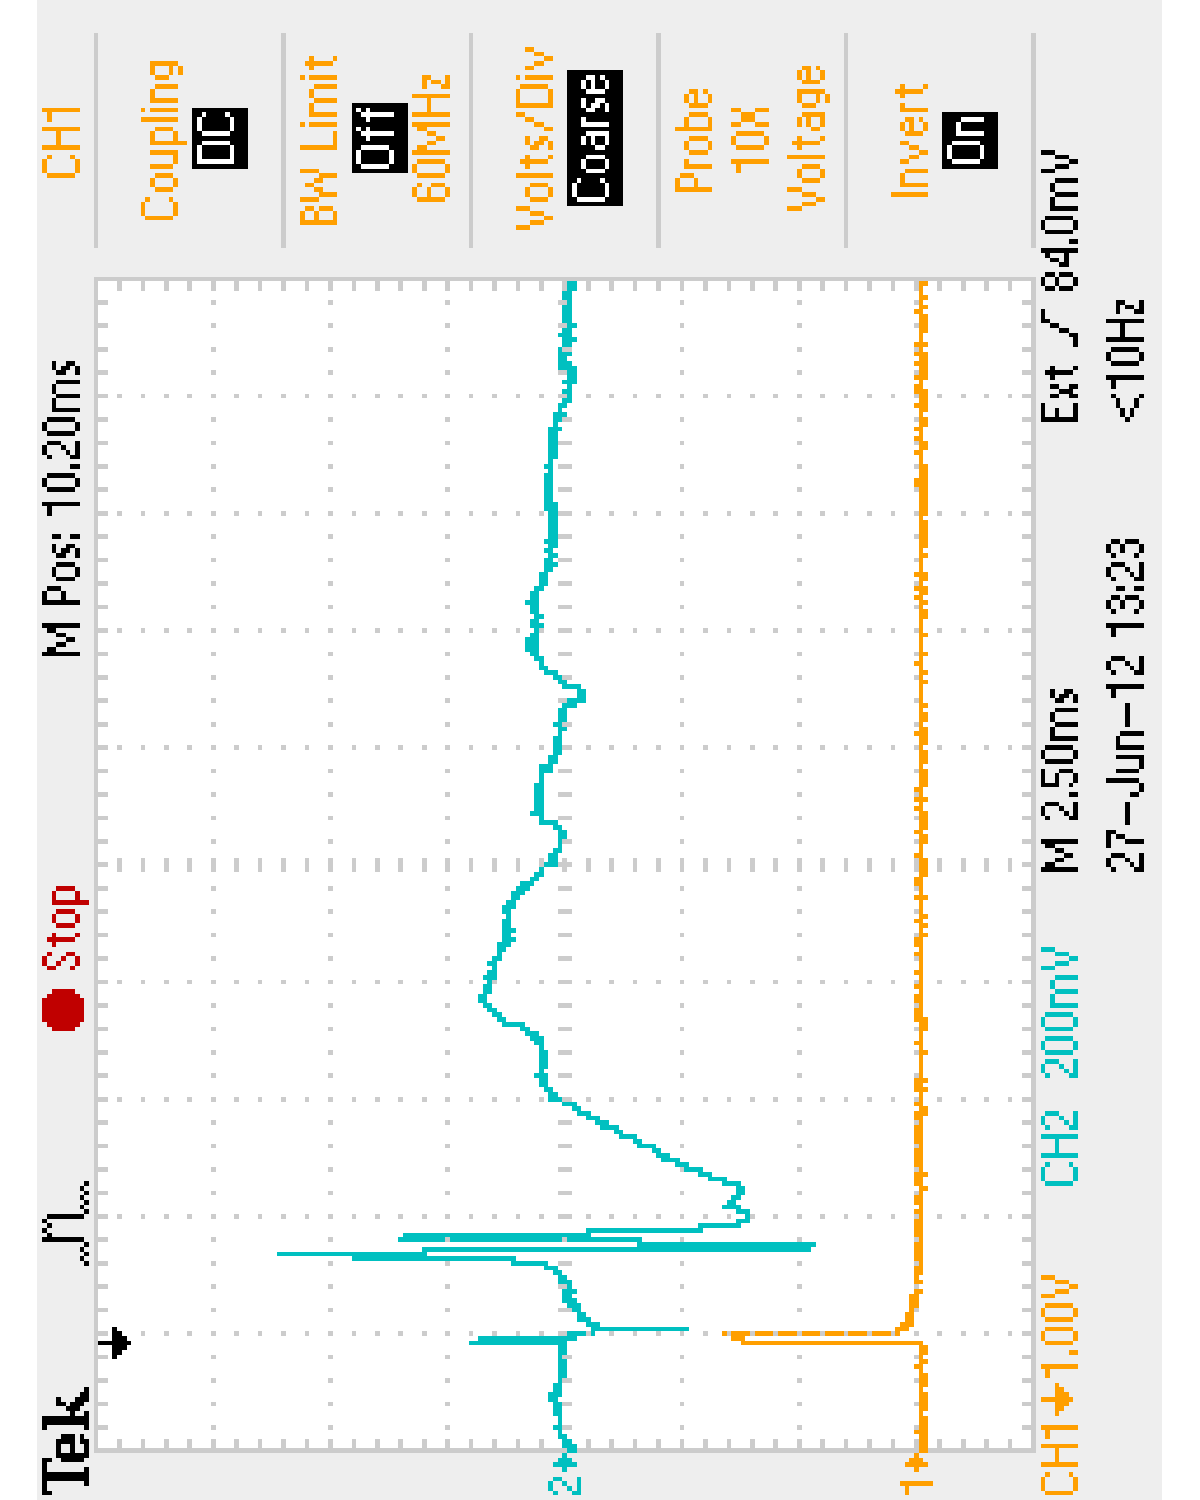
\includegraphics[trim=0 0.1in 0 0.1in,clip,clip,angle=-90,width=\textwidth]{./figures/F0001TEK_abnorm_120627} %[trim=left bottom right top]
	\caption{ALL0001 June 27, 2012}
	\end{subfigure}
	\caption{Abnormally shaped earthworm giant axon responses\label{fig:abnormal}}
	\end{singlespace}
\end{figure}

\begin{figure}[H]
	\centering 
	\begin{singlespace}
	\begin{subfigure}[b]{0.48\textwidth}
		\centering 
		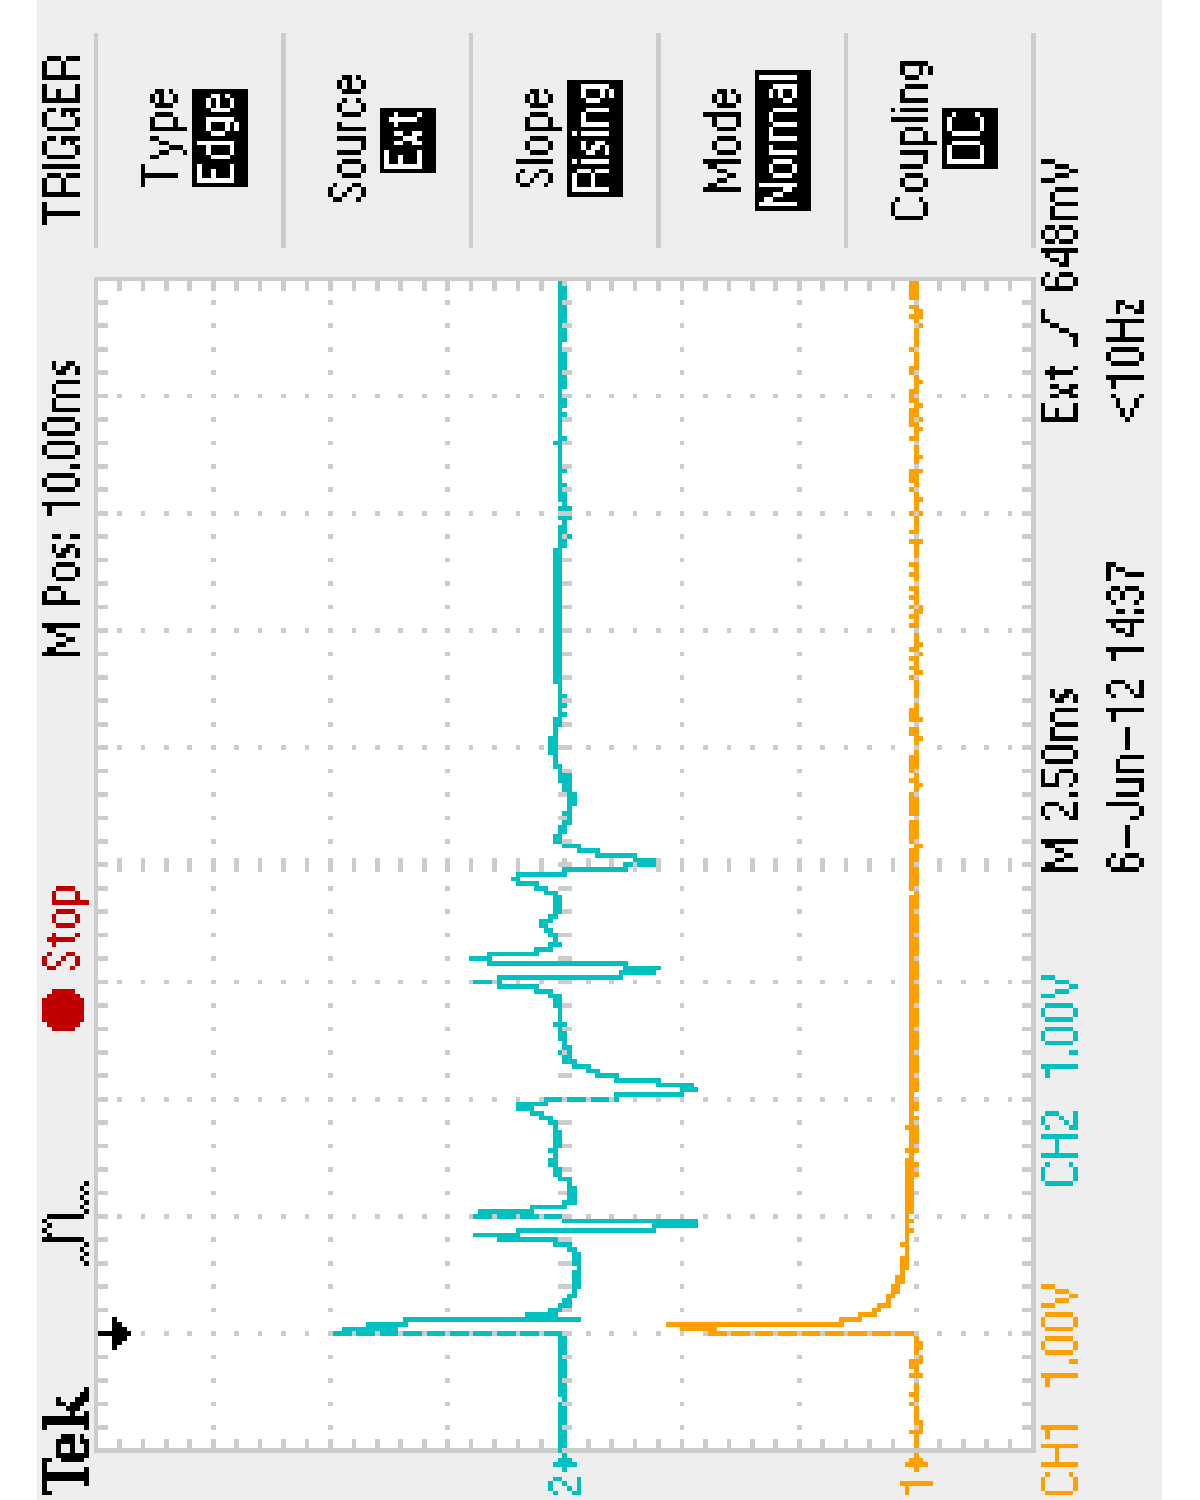
\includegraphics[trim=0 0.1in 0 0.1in,clip,angle=-90,width=\textwidth]{./figures/F0003TEK_multi_120606} %[trim=left bottom right top]
	\caption{ALL0003 June 06, 2012}
	\end{subfigure}
	~
	\begin{subfigure}[b]{0.48\textwidth}
		\centering 
		\resizebox{\textwidth}{!}{% GNUPLOT: LaTeX picture with Postscript
\begingroup
  \makeatletter
  \providecommand\color[2][]{%
    \GenericError{(gnuplot) \space\space\space\@spaces}{%
      Package color not loaded in conjunction with
      terminal option `colourtext'%
    }{See the gnuplot documentation for explanation.%
    }{Either use 'blacktext' in gnuplot or load the package
      color.sty in LaTeX.}%
    \renewcommand\color[2][]{}%
  }%
  \providecommand\includegraphics[2][]{%
    \GenericError{(gnuplot) \space\space\space\@spaces}{%
      Package graphicx or graphics not loaded%
    }{See the gnuplot documentation for explanation.%
    }{The gnuplot epslatex terminal needs graphicx.sty or graphics.sty.}%
    \renewcommand\includegraphics[2][]{}%
  }%
  \providecommand\rotatebox[2]{#2}%
  \@ifundefined{ifGPcolor}{%
    \newif\ifGPcolor
    \GPcolorfalse
  }{}%
  \@ifundefined{ifGPblacktext}{%
    \newif\ifGPblacktext
    \GPblacktexttrue
  }{}%
  % define a \g@addto@macro without @ in the name:
  \let\gplgaddtomacro\g@addto@macro
  % define empty templates for all commands taking text:
  \gdef\gplbacktext{}%
  \gdef\gplfronttext{}%
  \makeatother
  \ifGPblacktext
    % no textcolor at all
    \def\colorrgb#1{}%
    \def\colorgray#1{}%
  \else
    % gray or color?
    \ifGPcolor
      \def\colorrgb#1{\color[rgb]{#1}}%
      \def\colorgray#1{\color[gray]{#1}}%
      \expandafter\def\csname LTw\endcsname{\color{white}}%
      \expandafter\def\csname LTb\endcsname{\color{black}}%
      \expandafter\def\csname LTa\endcsname{\color{black}}%
      \expandafter\def\csname LT0\endcsname{\color[rgb]{1,0,0}}%
      \expandafter\def\csname LT1\endcsname{\color[rgb]{0,1,0}}%
      \expandafter\def\csname LT2\endcsname{\color[rgb]{0,0,1}}%
      \expandafter\def\csname LT3\endcsname{\color[rgb]{1,0,1}}%
      \expandafter\def\csname LT4\endcsname{\color[rgb]{0,1,1}}%
      \expandafter\def\csname LT5\endcsname{\color[rgb]{1,1,0}}%
      \expandafter\def\csname LT6\endcsname{\color[rgb]{0,0,0}}%
      \expandafter\def\csname LT7\endcsname{\color[rgb]{1,0.3,0}}%
      \expandafter\def\csname LT8\endcsname{\color[rgb]{0.5,0.5,0.5}}%
    \else
      % gray
      \def\colorrgb#1{\color{black}}%
      \def\colorgray#1{\color[gray]{#1}}%
      \expandafter\def\csname LTw\endcsname{\color{white}}%
      \expandafter\def\csname LTb\endcsname{\color{black}}%
      \expandafter\def\csname LTa\endcsname{\color{black}}%
      \expandafter\def\csname LT0\endcsname{\color{black}}%
      \expandafter\def\csname LT1\endcsname{\color{black}}%
      \expandafter\def\csname LT2\endcsname{\color{black}}%
      \expandafter\def\csname LT3\endcsname{\color{black}}%
      \expandafter\def\csname LT4\endcsname{\color{black}}%
      \expandafter\def\csname LT5\endcsname{\color{black}}%
      \expandafter\def\csname LT6\endcsname{\color{black}}%
      \expandafter\def\csname LT7\endcsname{\color{black}}%
      \expandafter\def\csname LT8\endcsname{\color{black}}%
    \fi
  \fi
  \setlength{\unitlength}{0.0500bp}%
  \begin{picture}(11520.00,8640.00)%
    \gplgaddtomacro\gplbacktext{%
      \colorrgb{0.00,0.00,0.00}%
      \put(1377,5044){\makebox(0,0)[r]{\strut{}-6}}%
      \colorrgb{0.00,0.00,0.00}%
      \put(1377,5535){\makebox(0,0)[r]{\strut{}-4}}%
      \colorrgb{0.00,0.00,0.00}%
      \put(1377,6026){\makebox(0,0)[r]{\strut{}-2}}%
      \colorrgb{0.00,0.00,0.00}%
      \put(1377,6518){\makebox(0,0)[r]{\strut{}0}}%
      \colorrgb{0.00,0.00,0.00}%
      \put(1377,7009){\makebox(0,0)[r]{\strut{}2}}%
      \colorrgb{0.00,0.00,0.00}%
      \put(1377,7500){\makebox(0,0)[r]{\strut{}4}}%
      \colorrgb{0.00,0.00,0.00}%
      \put(1377,7991){\makebox(0,0)[r]{\strut{}6}}%
      \colorrgb{0.00,0.00,0.00}%
      \put(1497,4844){\makebox(0,0){\strut{}0}}%
      \colorrgb{0.00,0.00,0.00}%
      \put(3282,4844){\makebox(0,0){\strut{}50}}%
      \colorrgb{0.00,0.00,0.00}%
      \put(5068,4844){\makebox(0,0){\strut{}100}}%
      \colorrgb{0.00,0.00,0.00}%
      \put(6853,4844){\makebox(0,0){\strut{}150}}%
      \colorrgb{0.00,0.00,0.00}%
      \put(8639,4844){\makebox(0,0){\strut{}200}}%
      \colorrgb{0.00,0.00,0.00}%
      \put(10424,4844){\makebox(0,0){\strut{}250}}%
      \colorrgb{0.00,0.00,0.00}%
      \put(917,6517){\rotatebox{90}{\makebox(0,0){\strut{}Voltage ($V$)}}}%
      \colorrgb{0.00,0.00,0.00}%
      \put(5960,4544){\makebox(0,0){\strut{}Time ($ms$)}}%
      \csname LTb\endcsname%
      \put(5960,8291){\makebox(0,0){\strut{}Multiple Stimulations}}%
    }%
    \gplgaddtomacro\gplfronttext{%
      \colorrgb{0.00,0.00,0.00}%
      \put(6139,5781){\makebox(0,0)[l]{\strut{}Stimulus Artifact}}%
      \put(6496,7254){\makebox(0,0)[l]{\strut{}Multiple Lateral Giant Responses?}}%
    }%
    \gplgaddtomacro\gplbacktext{%
      \colorrgb{0.00,0.00,0.00}%
      \put(1377,950){\makebox(0,0)[r]{\strut{}-6}}%
      \colorrgb{0.00,0.00,0.00}%
      \put(1377,1441){\makebox(0,0)[r]{\strut{}-4}}%
      \colorrgb{0.00,0.00,0.00}%
      \put(1377,1932){\makebox(0,0)[r]{\strut{}-2}}%
      \colorrgb{0.00,0.00,0.00}%
      \put(1377,2424){\makebox(0,0)[r]{\strut{}0}}%
      \colorrgb{0.00,0.00,0.00}%
      \put(1377,2915){\makebox(0,0)[r]{\strut{}2}}%
      \colorrgb{0.00,0.00,0.00}%
      \put(1377,3406){\makebox(0,0)[r]{\strut{}4}}%
      \colorrgb{0.00,0.00,0.00}%
      \put(1377,3897){\makebox(0,0)[r]{\strut{}6}}%
      \colorrgb{0.00,0.00,0.00}%
      \put(1497,750){\makebox(0,0){\strut{}-5}}%
      \colorrgb{0.00,0.00,0.00}%
      \put(3282,750){\makebox(0,0){\strut{}0}}%
      \colorrgb{0.00,0.00,0.00}%
      \put(5068,750){\makebox(0,0){\strut{}5}}%
      \colorrgb{0.00,0.00,0.00}%
      \put(6853,750){\makebox(0,0){\strut{}10}}%
      \colorrgb{0.00,0.00,0.00}%
      \put(8639,750){\makebox(0,0){\strut{}15}}%
      \colorrgb{0.00,0.00,0.00}%
      \put(10424,750){\makebox(0,0){\strut{}20}}%
      \colorrgb{0.00,0.00,0.00}%
      \put(917,2423){\rotatebox{90}{\makebox(0,0){\strut{}Voltage ($V$)}}}%
      \colorrgb{0.00,0.00,0.00}%
      \put(5960,450){\makebox(0,0){\strut{}Time ($ms$)}}%
      \csname LTb\endcsname%
      \put(5960,4197){\makebox(0,0){\strut{}Multiple Stimulations, Zoom}}%
    }%
    \gplgaddtomacro\gplfronttext{%
      \colorrgb{0.00,0.00,0.00}%
      \put(4443,1564){\makebox(0,0)[l]{\strut{}Stimulus Artifact}}%
      \put(5104,3222){\makebox(0,0)[l]{\strut{}Median Giant Response}}%
      \put(8728,2853){\makebox(0,0)[l]{\strut{}Lateral Giant Response?}}%
    }%
    \gplbacktext
    \put(0,0){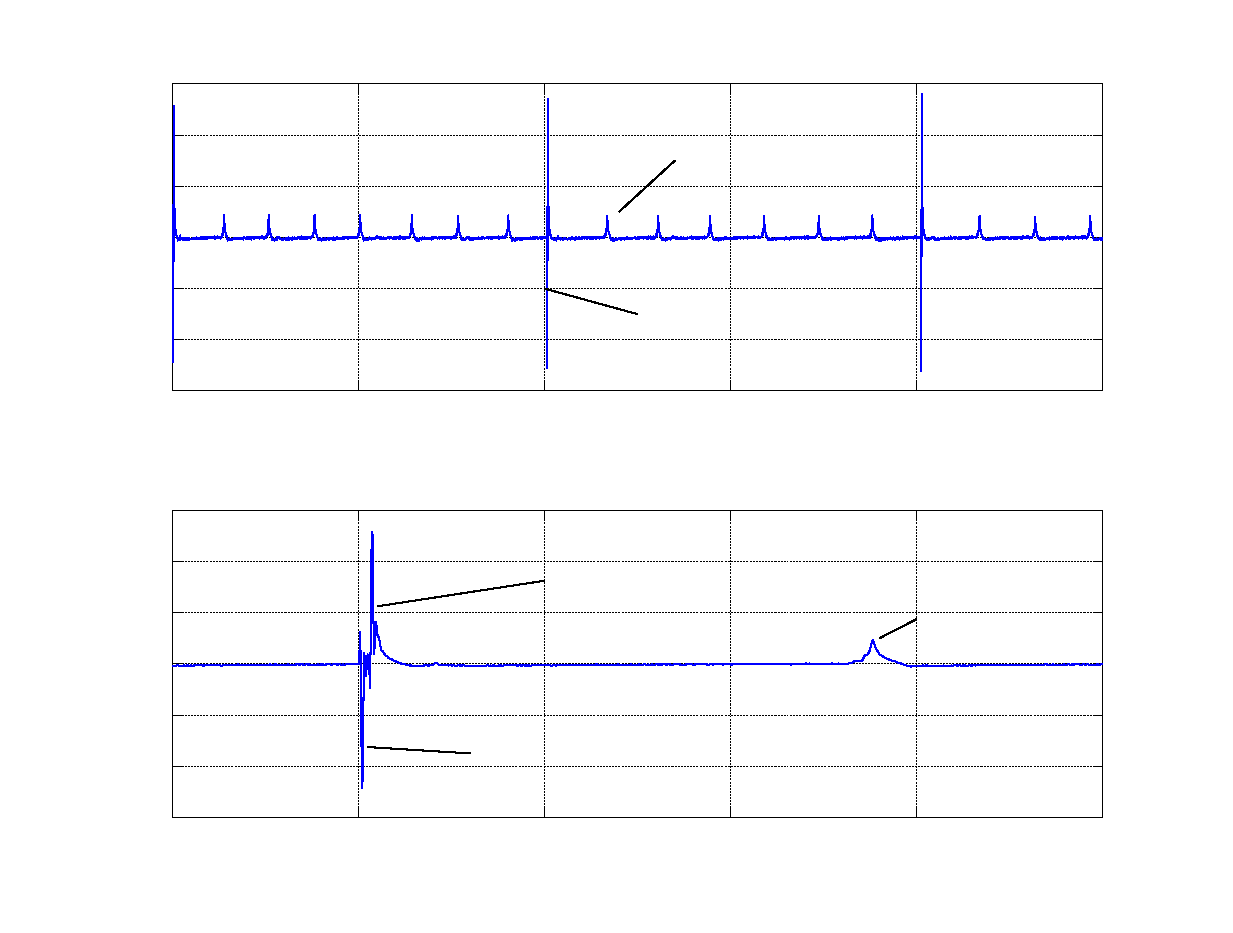
\includegraphics{MULTIresponse}}%
    \gplfronttext
  \end{picture}%
\endgroup
}
	\caption{data\_out0-multi1 May 16, 2012}
	\end{subfigure}
	\caption{Multiple earthworm giant axon responses per single stimulus\label{fig:multi}}
	\end{singlespace}
\end{figure}

\paragraph{Silver Wire Size} In an attempt to save money, larger diameter silver wire than is recommended in~\cite{KuehJellies} was used to perform the earthworm experiment.  The following is an excerpt from an email composed by me and sent to Dr.~Damon A.~Miller and Mr.~Mike Ellinger on April 22, 2012 summarizing the cost savings:

\begin{quotation}
For the silver wire,~\cite{KuehJellies} says to use 0.25mm diameter wire from Warner Instruments.  It looks like it can be bought here:  \url{http://www.warneronline.com/product_info.cfm?ID=280&CFID=6793639&CFTOKEN=40541278}

Their silver wire is 99.99\% pure, and under ``pricing and ordering,'' 2 meters of 0.25mm diameter wire costs \$24 not including shipping plus there's a \$10 charge for having an order of less than \$75.

I found another website that sells 99.99\% 0.635mm (0.025in) wire at \$3.00/ft.  Which means we could get 6ft. for \~\$24 including shipping or \~\$15 for 3ft.  Link: \url{http://www.ccsilver.com/silver/superfines.html}

Yet another website sells 6ft. of 99.9\% 0.025mm wire for \~\$10 including shipping.  Link: \url{http://www.ottofrei.com/store/product.php?productid=21270&cat=3847&page=1} (dead)

To sum up, we can get the original medical grade, 99.99\% purity wire in the same diameter for $>$\$35, we can get the same purity wire but with 2.5 times the diameter for \$15, or we can get 99.9\% wire in the same diameter as the experiment for \$10.

I'm thinking the 99.99\% 0.635mm wire for \$15 would be an acceptable solution.
\end{quotation}

Many of the anomalies in shape and amplitude mentioned in the previous section were observed while using the 0.635mm wire from C.C.~Silver for the recording electrodes.  To eliminate the wire diameter as a factor in those anomalies, the 0.25mm diameter wire from Warner Instruments specified by~\cite{KuehJellies} was purchased and compared with the 0.635mm wire.  Both wire sizes were chlorided and an earthworm was prepared.  The commercial stimulator was used along with a Preamp from~\cite{BatzerCorsiCrampton} connected to an oscilloscope.  Figure~\ref{fig:30to22} shows a 3.5V stimulation with response recorded first using the 0.25mm wire from Warner Instruments, then using the 0.635mm wire from C.C.~Silver.  Figure~\ref{fig:22to30} shows a 3.75V stimulation with response recorded first using the 0.635mm wire, then using the 0.25mm wire.

\begin{figure}[H]
	\centering 
	\begin{singlespace}
	\begin{subfigure}[b]{0.48\textwidth}
		\centering 
		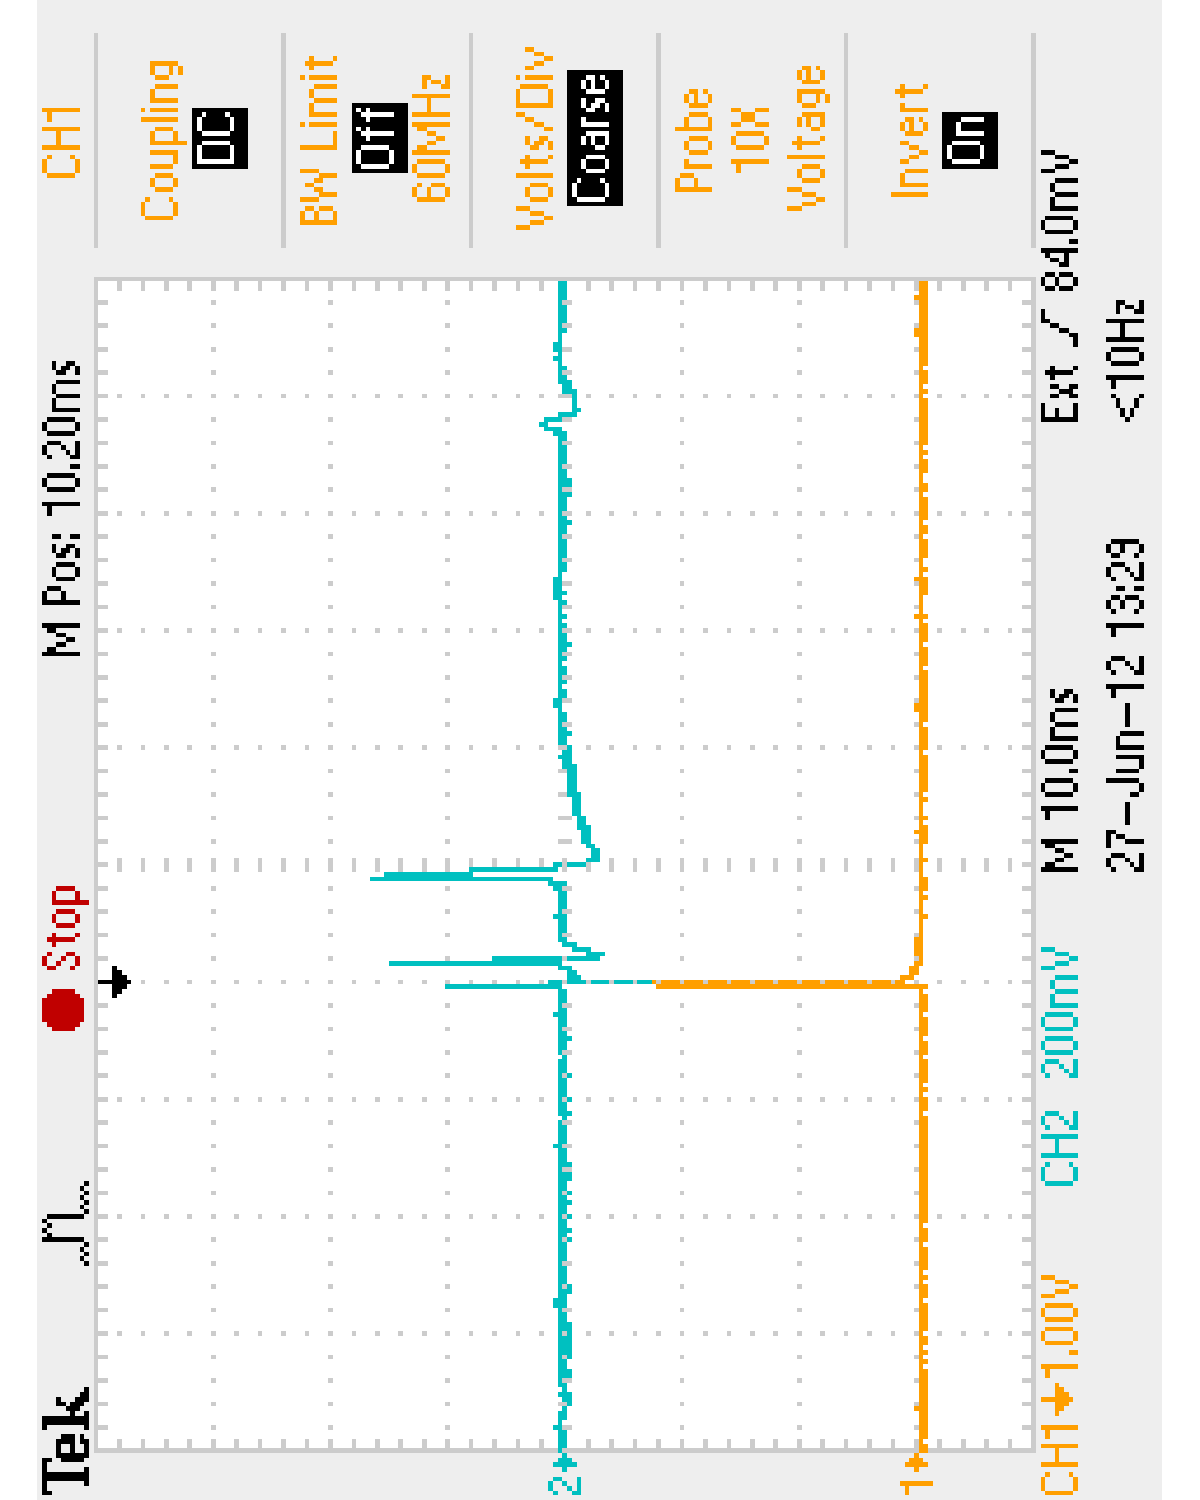
\includegraphics[trim=0 0.1in 0 0.1in,clip,angle=-90,width=\textwidth]{./figures/F0004TEK_30a_120627} %[trim=left bottom right top]
	\caption{ALL0004 June 27, 2012; 0.25mm wire; 3.5V stimulus}
	\end{subfigure}
	~
	\begin{subfigure}[b]{0.48\textwidth}
		\centering 
		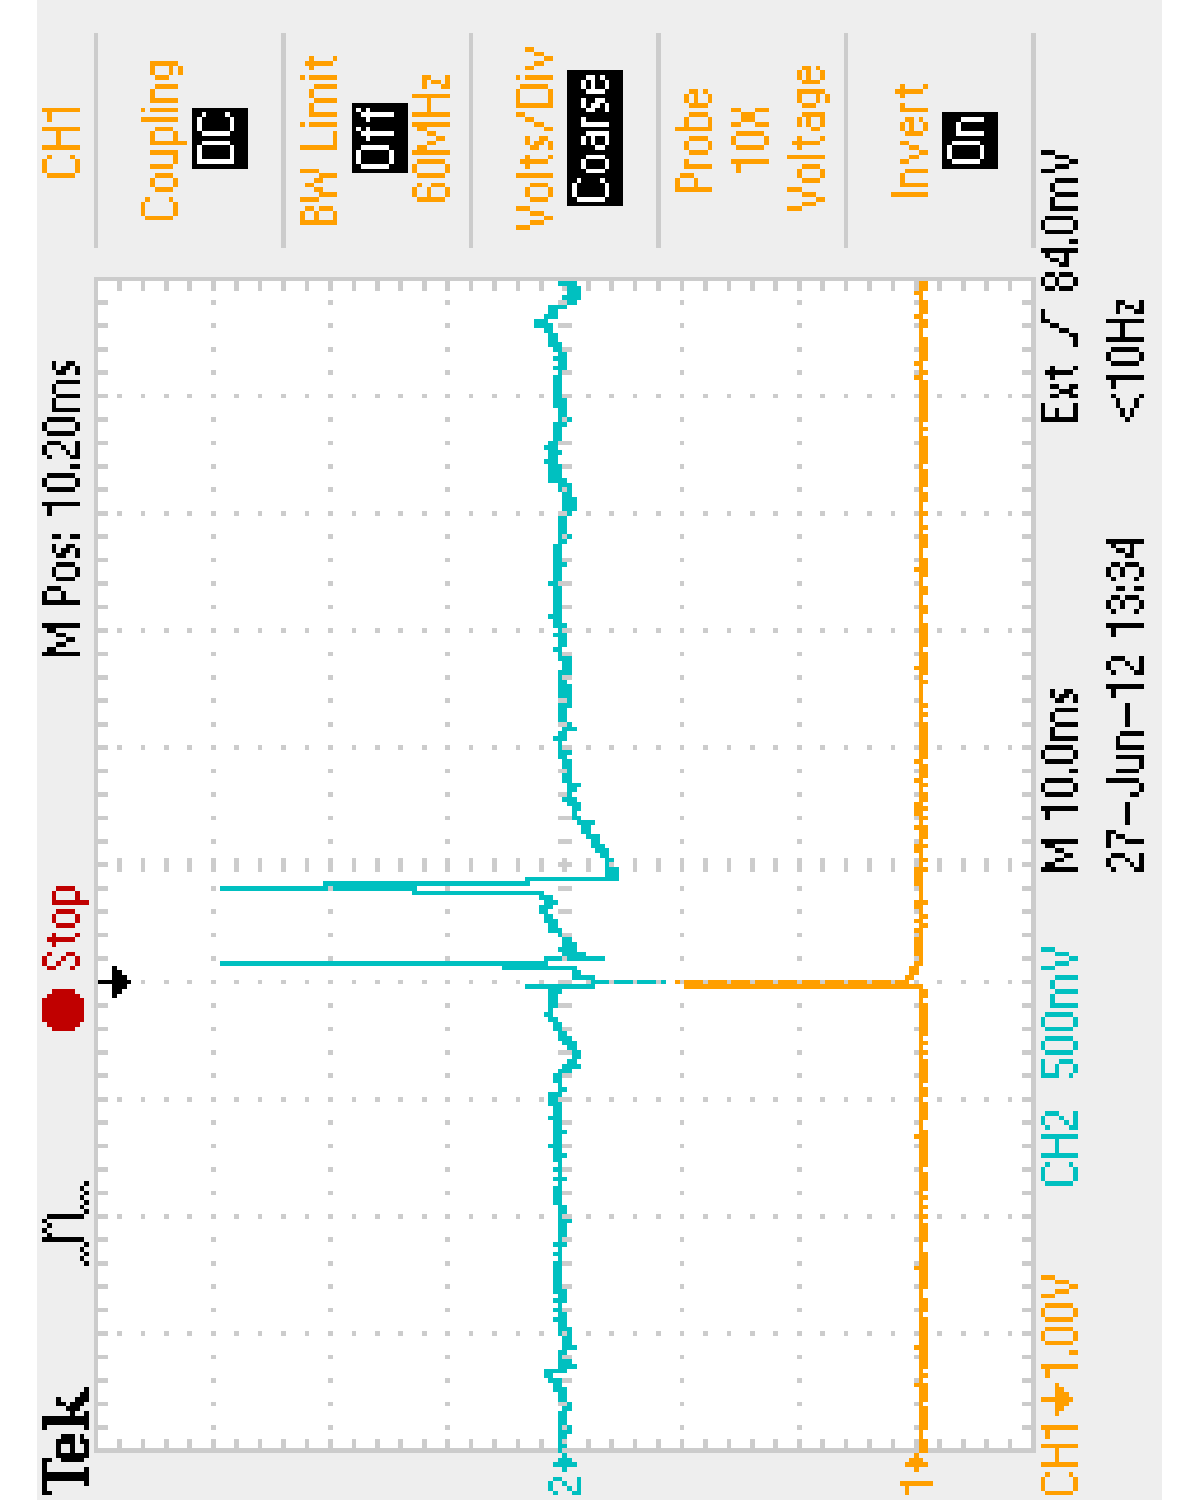
\includegraphics[trim=0 0.1in 0 0.1in,clip,angle=-90,width=\textwidth]{./figures/F0005TEK_22a_120627} %[trim=left bottom right top]
	\caption{ALL0005 June 27, 2012; 0.635mm wire; 3.5V stimulus}
	\end{subfigure}
	\caption{Recording electrode silver wire comparison: 0.25mm to 0.635mm\label{fig:30to22}}
	\end{singlespace}
\end{figure}
	
\begin{figure}[H]
	\centering 
	\begin{singlespace}
	\begin{subfigure}[b]{0.48\textwidth}
		\centering 
		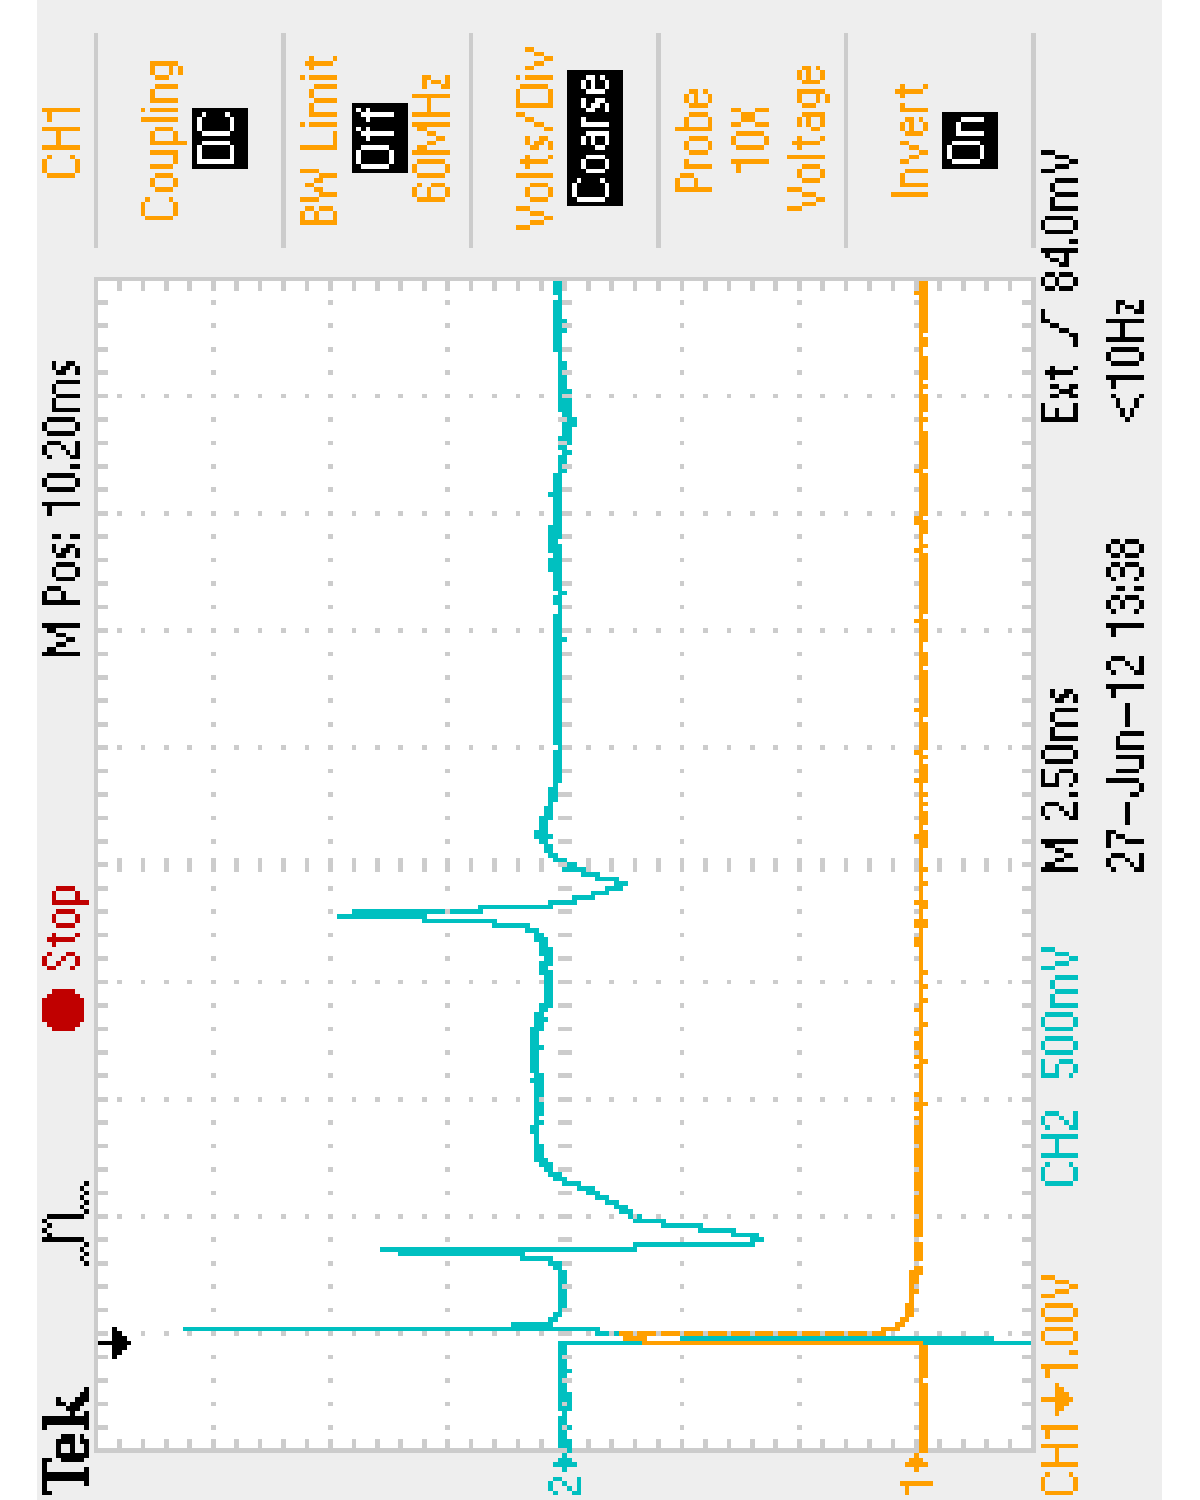
\includegraphics[trim=0 0.1in 0 0.1in,clip,angle=-90,width=\textwidth]{./figures/F0006TEK_22b_120627} %[trim=left bottom right top]
	\caption{ALL0006 June 27, 2012; 0.635mm wire; 3.75V stimulus}
	\end{subfigure}
	~
	\begin{subfigure}[b]{0.48\textwidth}
		\centering 
		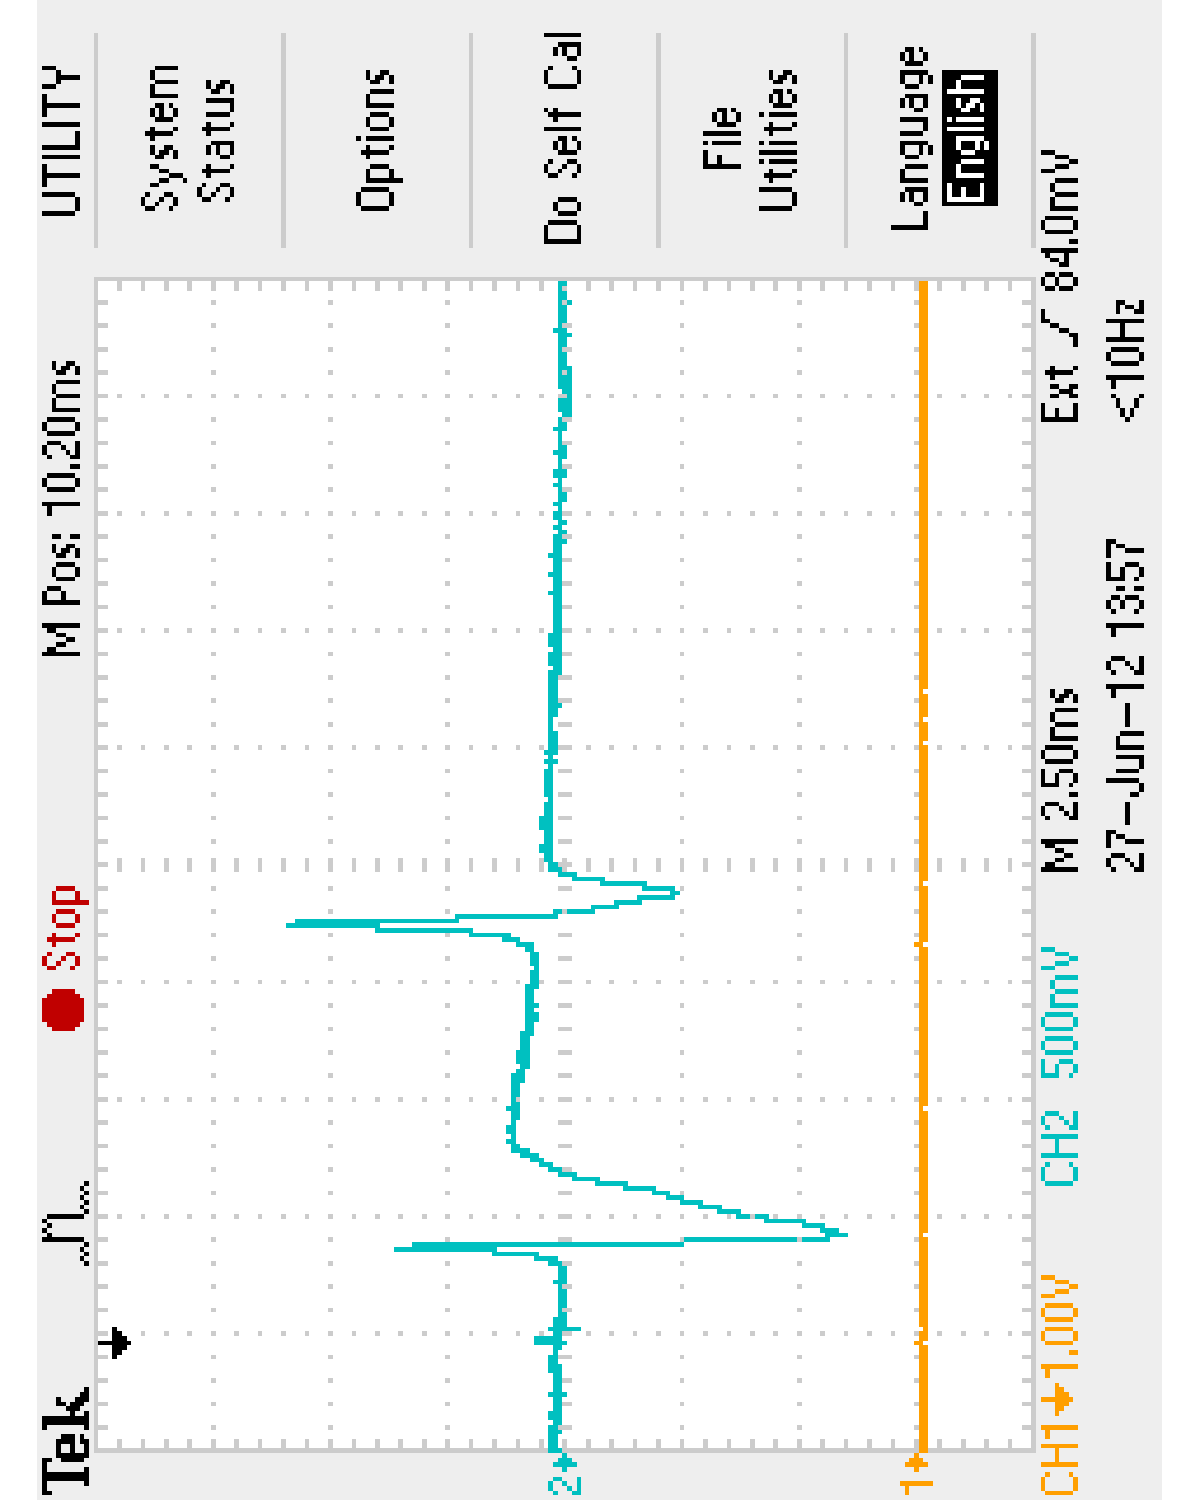
\includegraphics[trim=0 0.1in 0 0.1in,clip,angle=-90,width=\textwidth]{./figures/F0007TEK_30b_120627} %[trim=left bottom right top]
	\caption{ALL0007 June 27, 2012; 0.25mm wire; 3.5V stimulus}
	\end{subfigure}
	\caption{Recording electrode silver wire comparison: 0.635mm to 0.25mm\label{fig:22to30}}
	\end{singlespace}
\end{figure}

Anomalies in shape and amplitude were experienced with both diameter wires, during the experiment.  The figures show that similar shapes could be observed with both diameter wires.  This led me to the conclusion that wire diameter was not the cause of the difficulties examined in the previous section.
